\chapter{RISC-V Microprocessor Instruction Set Architecture}

\section{Overview of RISC-V}

Designing and developing a microprocessor, or Central Processing Unit (CPU), is a complex process requiring the collaboration of many experts in fields such as digital logic design, compiler development, and operating systems, along with significant financial resources. Major vendors like ARM, with prominent processor lines such as Cortex-M and Cortex-A, often impose high licensing fees and strict confidentiality requirements on their designs. This creates considerable barriers to hardware and software research and customization, particularly for academic institutions or small businesses. In response to these limitations, the RISC-V architecture \cite{waterman2014riscv, waterman2015riscvprivileged} was developed and introduced as an open-source solution, providing a flexible platform that eliminates licensing costs and allows for need-based customization. By fostering innovation and opening up a freer research ecosystem, RISC-V is reshaping the traditional approach to microprocessor development, aiming for more efficient and comprehensive solutions.

\begin{figure}[h!]
    \centering
    
\includegraphics[width=0.5\textwidth]{RISCV_Logo.pdf}
    \caption{RISC-V is managed by RISC-V International. Source \cite{riscv2024members}}
    \label{fig:riscv_international}
\end{figure}

Essentially, RISC-V is an open-source microprocessor instruction set architecture (ISA), designed and developed based on the Reduced Instruction Set Computer (RISC) methodology, and it represents the fifth generation of this design approach. For a program executing on a microprocessor, the RISC design methodology stipulates that the microprocessor executes only simple assembly (machine code) instructions, which have a fixed length and are executed within a single, uniform clock cycle. A complex task is performed by multiple assembly instructions, making the instruction set simple, compact, and easy to develop hardware for rapidly. This is entirely different from the Complex Instruction Set Computer (CISC) architecture, which aims to complete a task with the fewest possible assembly instructions. To achieve this, CISC microprocessors must be designed to execute structurally complex assembly instructions, capable of performing multiple specialized functions sequentially and executing over multiple clock cycles.

Originating as a project developed by researchers and graduate students at the University of California, Berkeley in 2010, the initial purpose of RISC-V was to create a practical ISA to support research and teaching in computer architecture, deployable on both hardware and software without licensing requirements. The original authors of RISC-V were individuals with considerable experience in computer design. Consequently, for stable development, RISC-V aimed for several goals, most of which have been achieved, including:
\begin{itemize}
    \item A complete, fully open-source ISA, free for academic, educational, and industrial use, with practical applicability suitable not only for experimental simulation but also for hardware implementation.
    \item An ISA not oriented towards complex microarchitectures or fixed by any specific implementation technology (FPGA, ASIC, full-custom, etc.) but still allowing for efficient implementation in any of these directions.
    \item An ISA divided into base ISAs, usable for developing hardware accelerators or for educational purposes, and optional standard extensions to support general software development.
    \item An ISA supporting extensive instruction set extensions with specialized functionalities and numerous variants.
    \item Support for the IEEE 754-2008 floating-point standard.
    \item Support for parallel, multi-core, and heterogeneous many-core implementations.
    \item Both 32-bit and 64-bit address space variants developed for applications, operating system kernels, and hardware implementations.
\end{itemize}

Due to its open-source nature, RISC-V allows developers to freely use the design architecture without paying intellectual property and licensing fees. This creates development opportunities for RISC-V itself as it is adopted by the research community and educational institutions, gradually becoming popular in industry, and attracting significant attention from many large companies, corporations, and even governments of various countries. Furthermore, designers using the RISC-V ISA can utilize it without limitations in both hardware and software. This means developers are encouraged, but not required, to publicly disclose their designs and projects developed using RISC-V.

Currently, the development process and rights regarding the publication, release, and maintenance of intellectual property and official documentation related to RISC-V are managed by RISC-V International, based in Switzerland. This meets the standardization requirements for designers and users for commercial purposes, who demand a system using the RISC-V ISA that can operate and exist for many years.

To suit various implementers and ensure flexibility in designs with specialized characteristics, the RISC-V instruction set is divided and standardized into two main parts: the base instruction set and standard extensions. The RISC-V instruction set supports 32-bit, 64-bit, and 128-bit architectures with the respective base instruction sets RV32I, RV32E, RV64I, and RV128I. Among these, RV32I is the most important and common set for 32-bit microprocessors, featuring 40 integer manipulation instructions. The fact that RISC-V only standardizes and provides the instruction set allows hardware designers the freedom to choose how to implement their designs.

\subsection{RISC-V 32-bit and the RV32I Base Instruction Set}

RV32I \cite{waterman2014riscv} is the base instruction set present in almost all 32-bit RISC-V microprocessor architectures. The assembly instructions in this set use 32 32-bit registers, named \texttt{x0} - \texttt{x31}, to store integers. Each register, in addition to being numbered from 0 to 31, is also referred to by its Application Binary Interface (ABI) name, which reflects its specific function. For example, register \texttt{x0} is a read-only register containing the constant value "0", and register \texttt{x1} is used as the return address register, storing the return address when a function is executed. Table \ref{tab:rv32i_registers} lists these registers and their functions in detail.

\begin{table}[h!]
    \centering
    \caption{ABI names and functions of registers in RV32I. Source \cite{waterman2014riscv}}
    \label{tab:rv32i_registers}
    \begin{tabular}{lll}
    \toprule
    Register & ABI Name & Description \\
    \midrule
    x0 & zero & Constant "0" \\
    x1 & ra & Return address \\
    x2 & sp & Stack pointer \\
    x3 & gp & Global pointer \\
    x4 & tp & Thread pointer \\
    x5 $\to$ x7 & t0 $\to$ t2 & Temporary \\
    x8 & s0/fp & Memory/frame pointer \\
    x9 & s1 & Memory \\
    x10, x11 & a0, a1 & Function parameter/return value \\
    x12 $\to$ x17 & a2 $\to$ a7 & Function parameter \\
    x18 $\to$ x27 & s2 $\to$ s11 & Memory \\
    x28 $\to$ x31 & t3 $\to$ t6 & Temporary \\
    \bottomrule
    \end{tabular}
\end{table}

The assembly instructions in RV32I use six different 32-bit instruction formats, depending on the function of the instruction. These include R, I, S, U formats, as well as two additional formats for immediate values: B and J. These formats are clearly shown in Figure \ref{fig:rv32i_formats}. Notably, the source registers (\texttt{rs1} and \texttt{rs2}) and the destination register (\texttt{rd}) are kept in the same position in most formats, simplifying instruction decoding. The only discernible difference lies in how \texttt{rs2}, \texttt{rd}, and immediate values are organized within the instruction.

\begin{figure}[h!]
    \centering
    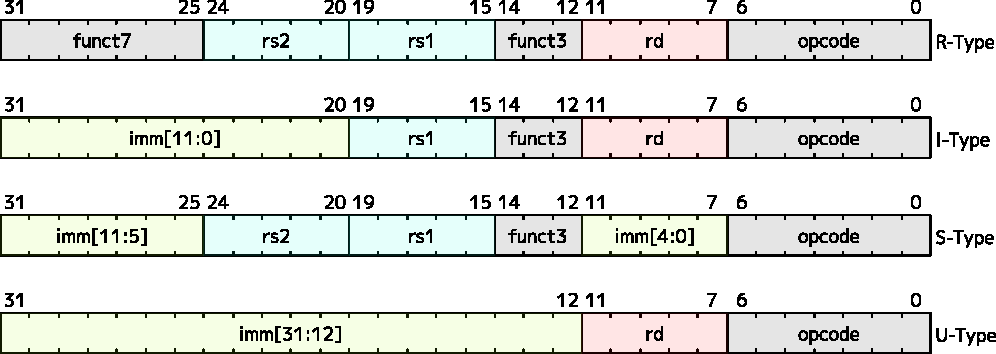
\includegraphics[width=\textwidth]{RISCV_BaseInstructionFormats.pdf}
    \caption{Instruction encoding formats in RV32I. Source \cite{waterman2014riscv}}
    \label{fig:rv32i_formats}
    \textit{Note: This figure should depict the R, I, S, U, B, and J formats as shown in the RISC-V specification.}
\end{figure}

Figure \ref{fig:rv32i_instructions} details all instructions in the RV32I base instruction set with their respective formats, specific opcode values, and function codes (\texttt{funct3} and \texttt{funct7}). Functionally, the RV32I set is divided into five distinct groups:
\begin{itemize}
    \item 21 integer computation instructions: Perform arithmetic (addition, subtraction, bit shifts), logic (AND, OR, XOR, NOT, etc.), and comparison operations on signed and unsigned numbers. Typically use R-type and I-type formats.
    \item 8 load-store instructions: LOAD and STORE byte, half-word, word (signed and unsigned), typically using I-type and S-type formats.
    \item 8 control-flow/branch instructions: Conditional branches, performing comparisons between two registers to decide whether to branch (BEQ/BNE, BLT, BGE), typically using I-type format.
    \item 2 system access instructions for the execution environment - ECALL and breakpoint - EBREAK, using I-type format.
    \item 1 memory access ordering instruction - FENCE, used by other processing cores (in multi-core scenarios) or other peripheral devices in the system. The I-type format is used for this instruction with some specific bit encoding rules and opcodes.
\end{itemize}

\begin{figure}[h!]
    \centering
    % \includegraphics[width=\textwidth]{rv32i_instruction_list_placeholder.png}
    \fbox{Placeholder for RV32I Instruction List Diagram}
    \caption{Instructions in the RV32I base instruction set. Source \cite{waterman2014riscv}}
    \label{fig:rv32i_instructions}
    \textit{Note: This figure should list the RV32I instructions as shown in the RISC-V specification.}
\end{figure}

With these 40 instructions, the microprocessor can perform most basic operations on integers. Additionally, several standard pseudo-instructions are defined to add tasks for which there are no dedicated instructions in the set. For example, the MOVE instruction - "\texttt{mv rd, rs}" - performs the function of moving/copying data between two registers. In a program, this instruction might be generated in the assembly code by a RISC-V compiler but is actually converted by assemblers into a standard instruction when translating to machine code, namely ADDI - Add Immediate "\texttt{addi rd, rs, 0}", which adds the source register to the constant "0" and assigns it to the destination register, achieving a similar function. Some other pseudo-instructions and their equivalent standard instructions are shown in Table \ref{tab:pseudo_instructions}.

\begin{table}[h!]
    \centering
    \caption{Pseudo-instructions and their corresponding standard instructions. Source \cite{waterman2014riscv}}
    \label{tab:pseudo_instructions}
    \begin{tabular}{lll}
    \toprule
    \textbf{Pseudo-instruction} & \textbf{Corresponding Core Instruction} & \textbf{Meaning} \\
    \midrule
    nop & addi rd, x0, x0 & No operation \\
    li rd, imm & addi rd, x0, imm & Load constant (immediate) \\
    mv rd, rs & addi rd, rs, 0 & Copy register \\
    not rd, rs & xori rd, rs, -1 & One's complement (invert) \\
    neg rd, rs & sub rd, x0, rs & Two's complement (negative) \\
    seqz rd, rs & sltiu rd, rs, 1 & Compare equal to zero \\
    snez rd, rs & sltiu rd, x0, rs & Compare not equal to zero \\
    sltz rd, rs & slt rd, rs, x0 & Compare less than zero \\
    sgtz rd, rs & slt rd, x0, rs & Compare greater than zero \\
    beqz rs, offset & beq rs, x0, offset & Branch if equal to zero \\
    bnez rs, offset & bne rs, x0, offset & Branch if not equal to zero \\
    blez rs, offset & bge x0, rs, offset & Branch if less than or equal to zero \\
    bgez rs, offset & bge rs, x0, offset & Branch if greater than or equal to zero \\
    bltz rs, offset & blt rs, x0, offset & Branch if less than zero \\
    bgtz rs, offset & blt x0, rs, offset & Branch if greater than zero \\
    j offset & jal x0, offset & Jump to label (offset) \\
    jal offset & jal x1, offset & Jump and link register \\
    ret & jalr x0, 0(x1) & Return from subroutine \\
    \bottomrule
    \end{tabular}
\end{table}

As mentioned, a goal of RISC-V is to support implementations requiring more features beyond the base instruction set. This is reflected in RISC-V defining extensions \cite{waterman2014riscv} for its instruction set architecture. These extensions define additional instruction encodings for various functionalities. For example, the standard M extension adds instructions for integer multiplication and division, while the standard F extension defines instructions for single-precision floating-point computation and manipulation.

\begin{table}[h!]
    \centering
    \caption{Development status of extended RISC-V instruction sets. Source \cite{waterman2014riscv}}
    \label{tab:extension_status}
    \begin{tabular}{llll}
    \toprule
    \textbf{Instruction Set} & \textbf{Function Description} & \textbf{Version} & \textbf{Status} \\
    \midrule
    M & Integer multiplication and division instruction set & 2.0 & Approved \\
    A & Atomic memory operation instruction set & 2.1 & Approved \\
    F & Single-precision floating-point computation & 2.2 & Approved \\
    D & Double-precision floating-point computation & 2.2 & Approved \\
    Q & Quad-precision floating-point computation & 2.2 & Approved \\
    C & Compressed instruction set & 2.0 & Approved \\
    Zifence & Instruction-Fetch Fence instruction set & 2.0 & Approved \\
    Zicsr & Control and Status Registers (CSRs) instruction set & 2.0 & Approved \\
    Ztso & Total Store Ordering instruction set & 1.0 & Approved \\
    \bottomrule
    \end{tabular}
\end{table}

Table \ref{tab:extension_status} above clearly lists the standard extension sets developed and published by RISC-V International. It can be seen that many instruction sets have been ratified and can be used in designs. When implemented, architectures supporting the RV32I base instruction set (or RV64I depending on the architecture) combined with the standard extensions M, A, F, D, Zicsr, and Zifencei are often summarized and referred to as the RV32G (or RV64G) instruction set, named for its general-purpose utility.

\subsection{RISC-V 64-bit and the RV64I Base Instruction Set}

Similar to RV32I, RV64I is the base instruction set for 64-bit microprocessor architectures, featuring 64-bit wide registers and supporting 64-bit addressing (XLEN=64), though instructions remain 32-bits wide. Architectures compliant with RV64I are compatible with RV32 instructions and include additional instructions to support operations between 32-bit and 64-bit data. For example, the \texttt{LW} instruction loads a 32-bit value and sign-extends it into a 64-bit register, while the new \texttt{LD} instruction loads a 64-bit word. The \texttt{ADD} instruction now performs 64-bit addition, while the \texttt{ADDW} instruction handles 32-bit addition, ignoring the upper 32 bits and returning a 32-bit signed value, sign-extended to 64 bits. These instructions enabling backward compatibility typically have a "W" suffix to denote 32-bit wide operations.

The compiler and calling conventions maintain the invariant that all 32-bit values are stored in sign-extended format within 64-bit registers. Even 32-bit unsigned integers will have bit 31 extended into bits 63 through 32. Consequently, converting between 32-bit signed and unsigned integers is a no-operation, as is converting from a 32-bit signed integer to a 64-bit signed integer. Existing 64-bit instructions like \texttt{SLTU} (set less than unsigned) and branch comparisons continue to operate correctly on 32-bit unsigned integers under this rule. Similarly, 64-bit logical operations on 32-bit sign-extended integers preserve the sign-extension property. A few new instructions (\texttt{ADD[I]W/SUBW/SxxW}) are necessary for addition and shifts to ensure reasonable performance for 32-bit values.

\begin{figure}[h!]
    \centering
    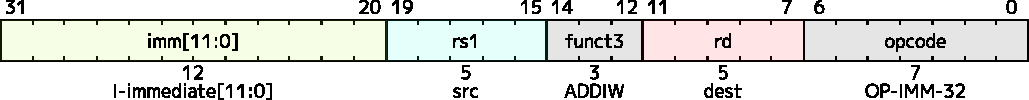
\includegraphics[width=0.8\textwidth]{RISCV_64bit_ADDIW.pdf}
    \caption{Instruction encoding format for ADDIW in 64-bit architecture. \cite{waterman2014riscv}}
    \label{fig:addiw_format}
\end{figure}

Some distinctly different instructions found only in RV64I include the \texttt{ADDIW} instruction, as shown in Figure \ref{fig:addiw_format}. \texttt{ADDIW} performs an addition between a 12-bit sign-extended immediate value and register \texttt{rs1}, producing a proper 32-bit sign-extended result in \texttt{rd}. Overflows are ignored, and the result consists of the lower 32 bits of the sum, sign-extended to 64 bits. Note, the instruction "\texttt{addiw rd, rs1, 0}" writes the sign-extension of the lower 32 bits of register \texttt{rs1} into register \texttt{rd} (pseudo-instruction \texttt{SEXT.W}).

\begin{figure}[h!]
    \centering
    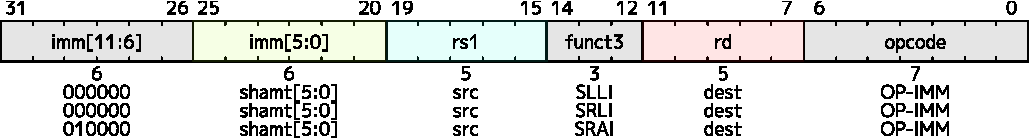
\includegraphics[width=0.8\textwidth]{RISCV_64bit_I_Type.pdf}
    \caption{Encoding format for 64-bit I-type shift instructions. \cite{waterman2014riscv}}
    \label{fig:rv64i_shift_i_format}
\end{figure}

I-type shift operations in RV64I (Figure \ref{fig:rv64i_shift_i_format}) use the same opcode as RV32I with some modifications. Register \texttt{rs1} contains the operand, and the shift amount is encoded in the lower 6 bits of the I-immediate field. Bit 30 determines the shift type: \texttt{SLLI} (logical left shift, zeros shifted into lower bits), \texttt{SRLI} (logical right shift, zeros shifted into upper bits), and \texttt{SRAI} (arithmetic right shift, sign bit copied into vacated upper bits).

\begin{figure}[h!]
    \centering
    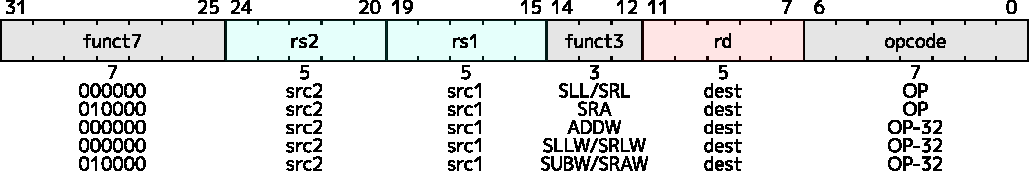
\includegraphics[width=0.8\textwidth]{RISCV_64bit_I_Type_ShiftBit.pdf}
    \caption{Encoding format for 64-bit R-type shift instructions for word operations. \cite{waterman2014riscv}}
    \label{fig:rv64i_shift_r_format}
\end{figure}

The \texttt{ADDW} and \texttt{SUBW} instructions in RV64I, similar to \texttt{ADD} and \texttt{SUB} for 64-bit operations, operate on 32-bit data and produce a 32-bit signed result, which is then sign-extended to 64-bits before being written to the destination register. Overflows are also ignored. The \texttt{SLL}, \texttt{SRL}, and \texttt{SRA} instructions perform logical left, logical right, and arithmetic right shifts on the value in \texttt{rs1}, with the shift amount determined by the lower 6 bits of \texttt{rs2}. The \texttt{SLLW}, \texttt{SRLW}, and \texttt{SRAW} instructions (Figure \ref{fig:rv64i_shift_r_format}), unique to RV64I, operate on 32-bit values and use the lower 5 bits of \texttt{rs2} to determine the shift amount.

Finally, load-store instructions can be mentioned. RV64I extends the address space to 64 bits, but the number of accessible addresses may vary depending on the execution environment.

\begin{figure}[h!]
    \centering
    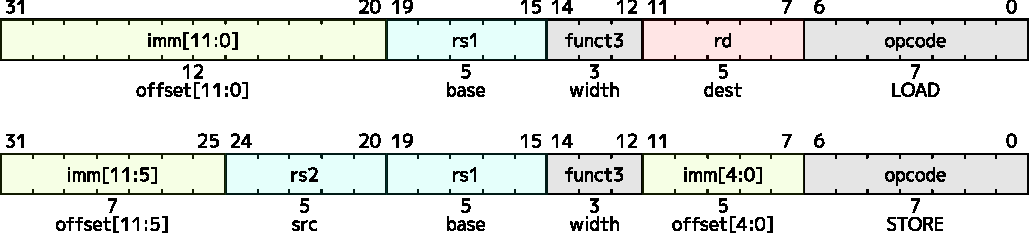
\includegraphics[width=\textwidth]{RISCV_64bit_LoadStoreWord.pdf}
    \caption{Encoding formats for 64-bit LOAD and STORE instructions. \cite{waterman2014riscv}}
    \label{fig:rv64i_load_store_format}
\end{figure}

The instruction formats are shown in Figure \ref{fig:rv64i_load_store_format}. The \texttt{LD} instruction here will load a 64-bit value, \texttt{LW} loads a 32-bit value (sign-extended to 64-bits) from memory into a register, and \texttt{LWU} zero-extends a 32-bit value from memory into register \texttt{rd}. Similarly, \texttt{LH/LHU} and \texttt{LB/LBU} handle 16-bit and 8-bit values. The \texttt{SD}, \texttt{SW}, \texttt{SH}, and \texttt{SB} instructions store 64-bit, 32-bit, 16-bit, and 8-bit values from register \texttt{rs2} to memory, respectively.

\subsection{RISC-V Processor Cores}

With its open-source nature, system developers can freely implement designs based on the RISC-V architecture, supported by an increasingly robust and growing ecosystem. The RISC-V ISA ecosystem mentioned here includes a diverse range of components from hardware design tools, low-level firmware development, bootloaders, to fully functional operating system kernels. Currently, development tools such as GCC/LLVM compilers, QEMU and Verilator simulators, and even the Linux operating system have incorporated RISC-V architecture and are under active development. As of the time of writing this thesis, there are over 100 open-source hardware processor cores and more than 40 open-source SoC platforms using the RISC-V ISA that have been and continue to be developed.

This section will provide a general overview of pipeline, in-order, and out-of-order architectures commonly implemented in microprocessors. Subsequently, a brief survey of open-source RISC-V processor cores will be conducted to select the most suitable design for implementation.

\subsection{Pipeline Architecture in Microprocessors}

A modern general-purpose CPU is often designed using a pipeline architecture. This technique draws inspiration from industrial assembly lines, dividing the processing of an assembly instruction into multiple stages or segments, each performed by different specialized hardware units connected sequentially throughout the process and capable of continuous operation. This architecture is commonly found in many microprocessor designs using RISC in general and RISC-V ISA in particular, due to its higher performance compared to processing instructions sequentially and waiting for results.

\begin{figure}[h!]
    \centering
    % \includegraphics[width=0.7\textwidth]{pipeline_stages_placeholder.png}
    \fbox{Placeholder for Pipeline Stages Diagram}
    \caption{Process of handling instructions through pipeline stages.}
    \label{fig:pipeline_stages}
\end{figure}

The concept of pipelining is illustrated in Figure \ref{fig:pipeline_stages}. While one assembly instruction is being processed in later stages, another assembly instruction begins processing in earlier stages, in parallel with previous instructions. It can be seen that at the fourth clock cycle, the pipeline is processing four different instructions in parallel, each in a distinct stage. A basic microprocessor pipeline consists of five stages. However, depending on the implementation and design, a microprocessor may use more or fewer stages, but still follows the sequence of stages explained below:
\begin{itemize}
    \item \textbf{Instruction Fetch (IF):} Retrieves instructions from the instruction memory, also known as program memory. Each instruction code that the CPU must execute is stored in the program memory. These instruction codes are binary sequences compiled from C/C++ code or assembly code.
    \item \textbf{Instruction Decode (ID):} The binary of each instruction is decoded, and corresponding control signals are activated.
    \item \textbf{Execute (EX):} Performs calculations and processing corresponding to the decoded instruction, such as addition, subtraction, multiplication, division, shifts, assignments, branches, etc.
    \item \textbf{Memory Access (MEM):} Accesses memory and performs read/write operations of data from/to memory.
    \item \textbf{Writeback (WB):} Saves the results after instruction execution to the location specified by the instruction, such as registers.
\end{itemize}

\subsection{Out-of-Order Architecture in Microprocessors}

Alternatively, out-of-order execution architecture is a crucial paradigm in modern CPU design, delivering significant performance gains by allowing instructions to be executed as soon as their input operands are ready, rather than strictly adhering to the program order as in a pipeline. This architecture is also a core element in high-performance systems used in scientific computing and artificial intelligence research. This flexible execution model addresses performance bottlenecks caused by data dependencies, cache latencies, and pipeline stalls, ensuring more efficient utilization of computational resources.

Key components of this architecture include the instruction window, which stores multiple instructions for dependency analysis, and dynamic scheduling mechanisms such as Tomasulo's algorithm or scoreboarding, which track dependencies and resource availability. Another critical feature is the Re-order Buffer (ROB), which helps maintain program order during instruction retirement, ensuring correct architectural state updates and precise exception handling. By decoupling instruction fetch and execution stages, out-of-order processors achieve higher instruction throughput and sustain the performance of execution units, optimizing efficiency across various applications.

Despite its many strengths and implementation benefits, out-of-order processors also present significant design challenges. The hardware blocks required for components like the ROB and branch prediction increase complexity, chip area, and power consumption, making energy efficiency optimization an important research area. Furthermore, extending out-of-order architecture to meet the demands of heterogeneous processing and large-scale parallel computing requires innovative approaches in dynamic scheduling and resource management.

\subsection{Open-Source RISC-V Processor Cores}

Rocket \cite{asanovic2016rocket}, or Rocket Core, is a RISC-V instruction set architecture microprocessor core designed by the Berkeley Architecture Research group. Rocket features a 5-stage, in-order architecture and implements the RISC-V RV32G and RV64G instruction sets.

\begin{figure}[h!]
    \centering
    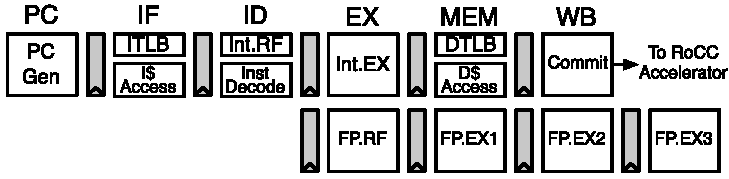
\includegraphics[width=0.7\textwidth]{Rocket_Core_Pipeline_5stages.pdf}
    \caption{Pipeline of Rocket core. Source \cite{asanovic2016rocket}}
    \label{fig:rocket_pipeline}
\end{figure}

The design of this microprocessor integrates many advanced features, including a Memory Management Unit (MMU) that supports virtual memory, enabling efficient memory access and address translation. Besides its role as a general-purpose microprocessor, Rocket also serves as a library of reusable components, including functional units, caches, Translation Lookaside Buffer (TLB), Page Table Walker (PTW), and Control and Status Registers (CSRs), which are reused in many other microprocessor designs. This makes Rocket Core a foundational component in Chipyard - RocketChip, allowing for the rapid development and creation of experimental systems ranging from simple to complex.

Rocket is considered the most prominent microprocessor core in the open-source RISC-V development community due to its well-updated and stably supported development documentation. It is built using Chisel, a relatively new hardware construction language based on Scala, employing an object-oriented approach similar to software development. Therefore, the flexibility of the system development process and the applicability of Rocket Core are very high, making it suitable for implementing multi-core systems.

Along with Rocket Core, the Berkeley Out-of-Order Machine (BOOM) \cite{celio2015boom, celio2016boom_spec} is also a prominent open-source RISC-V core, designed for high performance and out-of-order execution. Also developed within the microprocessor architecture research group at the University of California, Berkeley, BOOM is aimed at applications in advanced academic research and industry, featuring a flexible design and high operational performance. BOOM is also written in the Chisel language as a generator, like Rocket Core, allowing for rapid deployment and customization of the core according to the RV64GC RISC-V architecture. The latest version, SonicBOOM \cite{zhao2020sonicboom} (also known as BOOMv3), achieves a performance of 6.2 CoreMarks/MHz, capable of competing directly with high-performance commercial processor cores, setting a high standard for open-source processor design.

\begin{figure}[h!]
    \centering
    % \includegraphics[width=0.9\textwidth]{boom_architecture_placeholder.png}
    \fbox{Placeholder for BOOM Architecture Diagram}
    \caption{Berkeley Out-of-Order Machine Processor Architecture. Source \cite{celio2015boom}}
    \label{fig:boom_architecture}
\end{figure}

Structurally, BOOM features a 10-stage pipeline architecture including Fetch, Decode, Register Rename, Dispatch, Issue, Register Read, Execute, Memory, Writeback, and Commit. These stages allow for detailed control and optimization of the instruction flow, maintaining the "out-of-order" functionality at the high speeds necessary for modern processors. Specifically, each stage performs as follows:
\begin{itemize}
    \item \textbf{Fetch:} Instructions are fetched from instruction memory and stored in a fetch buffer to prepare for processing.
    \item \textbf{Decode:} Instructions are converted into simpler micro-ops to optimize execution within the pipeline.
    \item \textbf{Register Rename:} Logical registers in the ISA are renamed to independent physical registers, reducing data conflicts and increasing processing efficiency.
    \item \textbf{Dispatch:} Micro-ops from the decode stage are sent to the Issue window, awaiting necessary operands.
    \item \textbf{Issue:} Instructions in the Issue window are checked for operand readiness, and when conditions are met, micro-ops are sent to an execution unit.
    \item \textbf{Register File (RF) Read:} Micro-ops read operands from the physical register file or bypass network, preparing data for the next stage.
    \item \textbf{Execute:} Micro-ops are processed by functional units, performing computational tasks and memory address calculations.
    \item \textbf{Memory:} Manages memory operations via Load Address Queue (LAQ), Store Address Queue (SAQ), and Store Data Queue (SDQ), performing loads when addresses are ready and stores when both address and data are available.
    \item \textbf{Writeback:} Results from operations are written back to the physical register file, ensuring updated values are stored for future instructions.
    \item \textbf{Commit:} The Reorder Buffer tracks the status of instructions in the pipeline and commits results when instructions complete, including storing data to memory.
\end{itemize}

Similar to Rocket Core, this is also considered one of the most prominent open-source microprocessor cores. However, BOOM's design is more geared towards ASIC implementation, and its numerous features along with the use of Chisel for implementation might pose difficulties in creating a multi-core design in Verilog and deploying it on FPGAs.

\subsection{Chipyard - Rocket Chip}

The Rocket Chip project, also developed by the Berkeley Architecture Research (BAR) group at the University of California, Berkeley, marked a significant advancement in open-source processor design. This project provides a flexible, scalable, and configurable platform, enabling the creation of custom RISC-V microprocessors tailored to diverse performance and application requirements. Rocket Chip is essentially a library of hardware generators that can be configured and interconnected in various ways, producing diverse SoC designs. This library can generate an in-order core (Rocket) or an out-of-order core (BOOM), and these cores can be connected to co-processors via an interface named RoCC (Rocket Custom Coprocessor) \cite{asanovic2016rocket}.

\begin{figure}[h!]
    \centering
    
\includegraphics[width=0.7\textwidth]{Chipyard_ChipyardLogo.pdf} 
    \caption{Chipyard, developed by UC Berkeley. Source: \cite{zhao2021chipyard}}
    \label{fig:chipyard_ucb}
\end{figure}

Subsequently, to develop and expand the capabilities of Rocket Chip, Chipyard was created. Chipyard is an open-source framework that integrates system design, simulation, and implementation for SoC development, and it has become one of the most actively embraced and developed frameworks by the community. Chipyard, also originating from UC Berkeley, is the result of continuous development and integration of Chisel, Rocket Chip, and the Rocket Core.

\begin{figure}[h!]
    \centering
    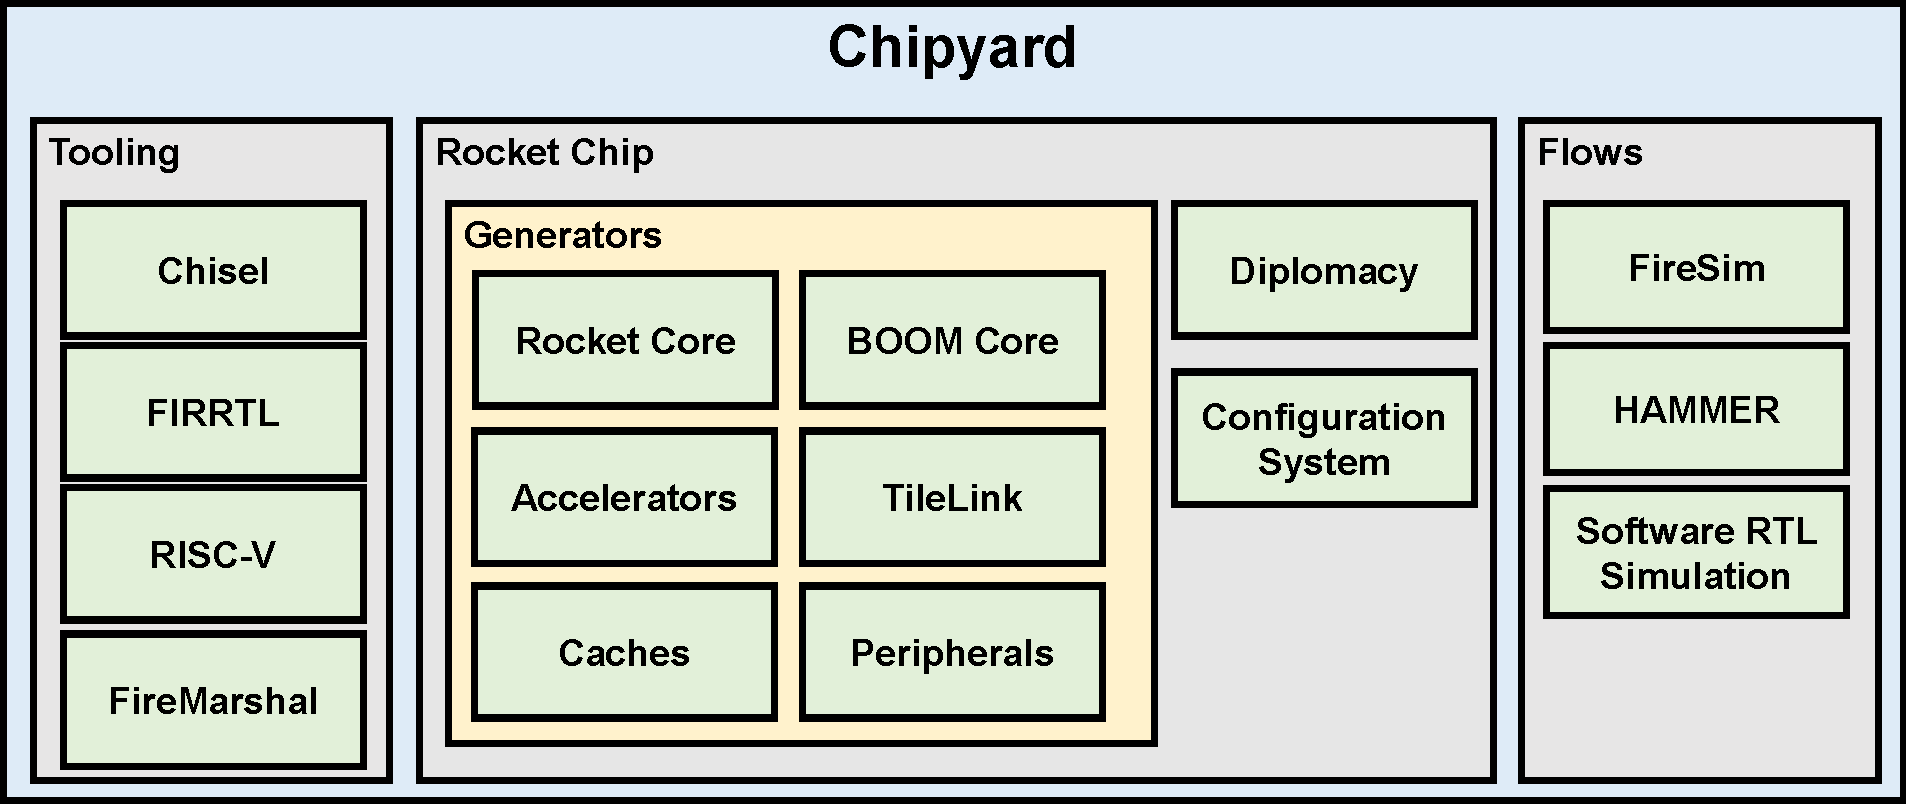
\includegraphics[width=0.8\textwidth]{Chipyard_Toolchain.pdf} % Replace placeholder.png with your actual image file
    \caption{Component structure of Chipyard. Source: \cite{zhao2021chipyard}}
    \label{fig:chipyard_structure}
\end{figure}

By utilizing Chisel, the FIRRTL compiler, the Rocket Chip generator, and other tools, Chipyard facilitates the development of highly customizable RISC-V SoCs. Chipyard includes a diverse set of processor cores (Rocket Core, BOOM, Ariane), accelerators (Hwacha, Gemmini, SHA3), along with comprehensive memory systems, peripheral devices, and tools to support the construction of a full-featured SoC. Chipyard supports multiple development flows, allowing for flexible hardware extension and experimentation. These development flows include software-based Register Transfer Level (RTL) simulation, FPGA-accelerated simulation using FireSim, automated VLSI flows with Hammer, and FireMarshal, which enables the creation and loading of software on both bare-metal systems (similar to microcontrollers) and Linux-based systems.

Rocket Chip supports deployment on FPGAs, with operational frequencies reaching 25-100 MHz depending on the configuration and the type of FPGA used. Currently, Rocket Chip is being utilized by SiFive \cite{sifive2024portfolio}, a company founded by some of the authors of RISC-V. SiFive produces RISC-V processors on silicon based on Rocket and provides tools for developing, testing, and evaluating their designs.

Using Chipyard (or Rocket Chip) as a foundation for system construction can pose several challenges due to its complexity in terms of the number of components and the design language used—Chisel. However, overcoming this barrier yields numerous benefits due to Rocket Chip's high flexibility and system customization capabilities. Its components are developed independently, have detailed development documentation, and are easily extensible. Furthermore, the Rocket Chip support community is very active, with more frequent updates and improvements compared to other frameworks.
